\section{Approach}
\label{sec:approach}
Let us define as \emph{actor} each person present in a 360º video. Therefore, the goal of our approach is to place subtitles based on the actors' position on a given 360° video. To accomplish this goal, we use face detection and clustering mechanisms to identify the actors' trajectory 360° video. Then, based on this trajectory, we place dynamic subtitles following the actors' path. For didatic purposes, we decided to divide our exposition in three phases: (i)~\emph{face detection in 360° videos}, (ii)~\emph{actors clusterization}, and (iii)~\emph{dynamic subtitles positioning}. These phases are described in the following subsections. 

\subsection{Face Detection in 360° videos}

In this phase, we aim at detecting the actors' faces present in the 360° video frames using object detection models.
%%
In general, an object detection model can identify which, among a known set of objects, are present in the image, and provides information about their positions with bounding boxes.
%%
Bounding boxes are specified by the $x$ and $y$ axes coordinates of the upper-left corner and of the lower-right corner of the rectangle that establishes the visual limits that encapsulate each object.
%%
In our case, objects are faces and, therefore, the face detection model is responsible for returning the position of the faces in an image~(video frame).
%%

Because of the distortions present on the equirectangular projection, we opted for elaborating a solution based on viewports extraction. A viewport is defined by its center, in polar coordinates~(lat, long), and its field of view~(FoV). Figure \ref{fig:viewports} shows viewports extracted at different polar coordinates from Figure \ref{subfig:out_equi}.

\begin{figure}[!ht]
    \centering
    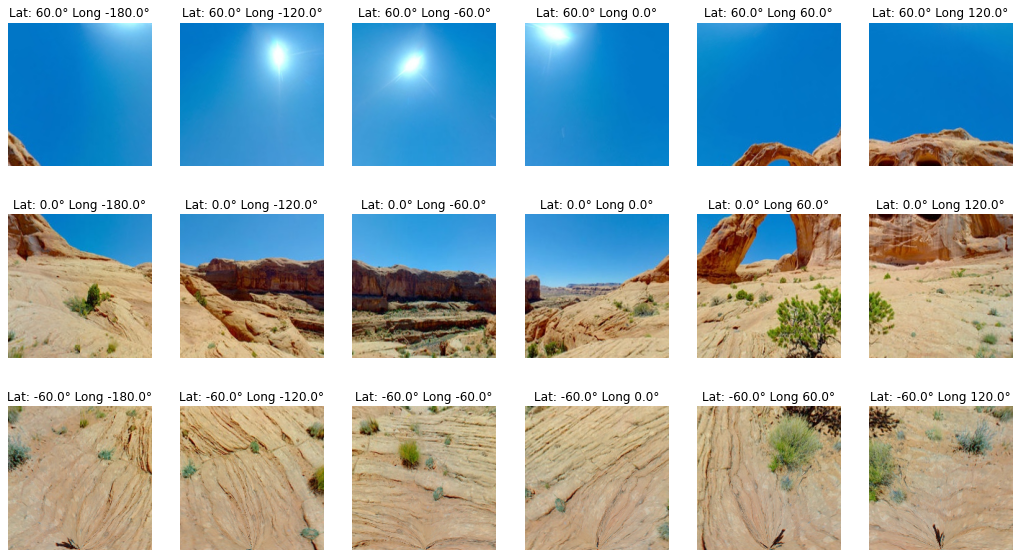
\includegraphics[width=1\textwidth]{img/viewports.png}
    \caption{Viewports extracted at different polar coordinates with $FoV = 60^{\circ}$}
    \label{fig:viewports}
\end{figure}

For each viewport, we apply a face detection model. 
Then, we project the faces detected bounding boxes back to the equirectangular image. For doing that for a given bounding box, we project the four corners and the mean point of each edge~(8 points in total). Therefore, in the equirectangular image, we deal with polyogons instead of bounding boxes, due to the distortions introduced. As different viewports may intersect and cover part of the same region in an image, we apply Non-maximum Supression~(NMS), eliminating intersected detections within a given threshold. One of the main advantages of this approach is that we can use face detection models trained in regular images, since distortions are reduced with the use of viewports.

Due to the lack of datasets for face detection in equirectangular images, we created a synthetic dataset based on the FDDB dataset~\cite{fddbTech}, a popular benchmark for face detection evaluation containing 2845 images and 5171 faces. We collected 19 indoor and outdoor equirectangular images, from Google Images,\footnote{https://www.google.com/imghp} ESO,\footnote{https://www.eso.org/public} and PxHere.\footnote{https://pxhere.com}
For each image in the FDDB dataset, we randomly chose a latitude, longitude and equirectangular image to project it. For each face present on that image, we projected the bounding box to a polygon exactly as mentioned in the viewport process. Figure \ref{fig:fddb_proj} shows an example of an image from FDDB projected in the polar coordinates \emph{lat} $ = -60^{\circ}$ \emph{long} $= 0^{\circ}$ to an equirectangular image.

\begin{figure}[!ht]
\centering
    \begin{subfigure}{0.4\linewidth}
        \centering
        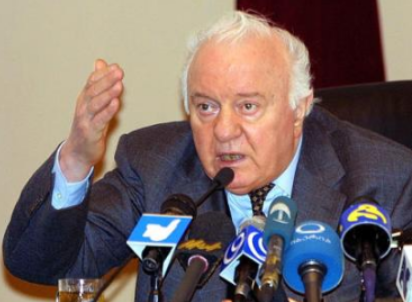
\includegraphics[height=10em]{img/face_pre.png}
        \caption{FDDB image example.}
        \label{subfig:face_pre}
    \end{subfigure}\hfill
    \begin{subfigure}{0.55\linewidth}
        \centering
        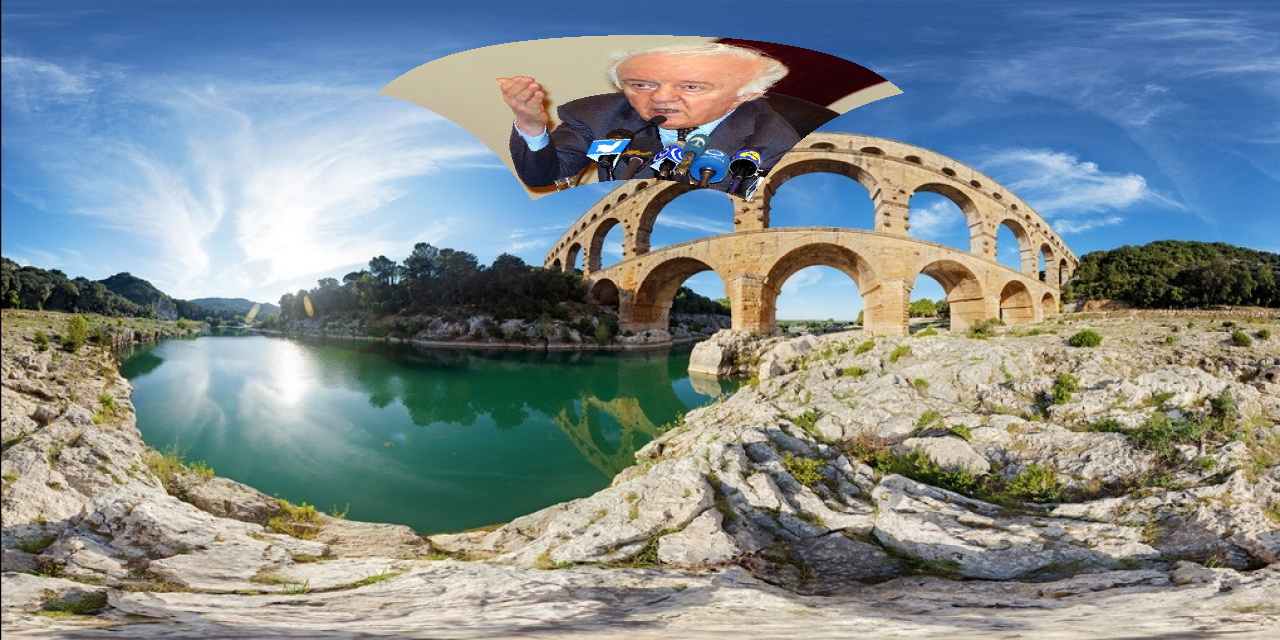
\includegraphics[height=10em]{img/face_pos.png}
        \caption{Projection example of FDDB image.}
        \label{subfig:face_pos}
    \end{subfigure}

\caption{FDDB image projection to Equirectangular image.}
\label{fig:fddb_proj}
\end{figure}

As evaluation metric, we intend to use Mean Average Precision~(mAP), that is commonly used to evaluate object detection algorithms~[ref]. As face detector, we are currently implementing a solution using MTCNN~\cite{mtcnn} (Multitask Cascaded Convolutional Networks) which is widely used for the face detection task~\cite{mtcnn1, mtcnn2, mtcnn3}. %If we have time, we also intend to test YOLO

In summary, for this phase, we have defined the following tasks:

\begin{itemize}
    \item \textbf{T 1.1}: Implementation of model based on viewports for face detection in 360° equirectangular images.
    \item \textbf{T 1.2}: Synthetic dataset creation.
    \item \textbf{T 1.3}: Model test in the dataset using MTCNN.
    \item \textbf{T 1.4}: Results evaluation using mAP.
\end{itemize}


\subsection{Actors Clusterization}



\subsection{Dynamic Subtitles Positioning}

